\documentclass[tikz,border=2pt]{standalone}
\usepackage{amsmath,amssymb}
\usepackage{tikz}
\usetikzlibrary{arrows.meta}

\begin{document}
% Complementary slackness lambda_i c_i(x*) = 0: either the constraint is active (c_i = 0) and
% may carry a positive multiplier, or it is inactive (c_i < 0) and its multiplier must vanish.
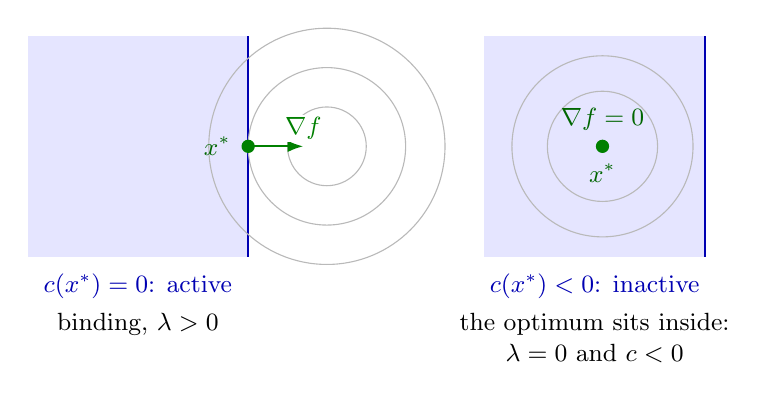
\begin{tikzpicture}[every node/.style={font=\small}, >={Latex[length=2mm]}, lab/.style={font=\small, fill=white, inner sep=1pt}]
	\begin{scope}
		\fill[blue!10] (-0.2,-0.2) rectangle (2.6,2.6);
		\draw[blue!70!black, thick] (2.6,-0.2) -- (2.6,2.6);
		\foreach \r in {0.5,1.0,1.5} {\draw[gray!55] (3.6,1.2) circle (\r);}
		\draw[->, green!50!black, thick] (2.6,1.2) -- (3.3,1.2) node[above, lab, yshift=1pt] {$\nabla f$};
		\fill[green!50!black] (2.6,1.2) circle (2.4pt);
		\node[green!40!black, font=\small, anchor=east] at (2.5,1.2) {$x^\ast$};
		\node[blue!70!black, font=\small, anchor=north] at (1.2,-0.3) {$c(x^\ast)=0$: active};
		\node[anchor=north] at (1.2,-0.8) {binding, $\lambda>0$};
	\end{scope}
	\begin{scope}[xshift=5.8cm]
		\fill[blue!10] (-0.2,-0.2) rectangle (2.6,2.6);
		\draw[blue!70!black, thick] (2.6,-0.2) -- (2.6,2.6);
		\foreach \r in {0.7,1.15} {\draw[gray!55] (1.3,1.2) circle (\r);}
		\fill[green!50!black] (1.3,1.2) circle (2.4pt);
		\node[green!40!black, font=\small, anchor=south] at (1.3,1.28) {$\nabla f=0$};
		\node[green!40!black, font=\small, anchor=north] at (1.3,1.1) {$x^\ast$};
		\node[blue!70!black, font=\small, anchor=north] at (1.2,-0.3) {$c(x^\ast)<0$: inactive};
		\node[anchor=north, align=center, font=\small] at (1.2,-0.8) {the optimum sits inside:\\ $\lambda=0$ and $c<0$};
	\end{scope}
\end{tikzpicture}
\end{document}
